\chapter{Conclusiones} \label{cap:conclusiones}

\section{Conclusiones}
A lo largo del desarrollo del Trabajo de Fin de Grado hemos pasado por numerosas versiones con distintos enfoques aplicados a la generación de bot de Ms. Pac-Man a través de gramáticas evolutivas. 
 
Primero de todo, mediante la generación de autómatas que ejecutaban cadenas de acciones (que posteriormente fue ampliado con acciones de más alto nivel y condicionales muy simples), que, si bien no alcanzó resultados destacablemente positivos, si logró encontrar una brecha en las reglas del juego que le permitía conseguir completar niveles muy fácilmente contra fantasmas no muy inteligentes.
 
Después, orientamos nuestra gramática a la generación de controladores reactivos, sustituyendo también las anteriores cadenas de acciones por un árbol de decisión. Este cambio supuso una mejora significativa, permitiéndonos diseñar gramáticas de distintos niveles de abstracción.
 
A continuación, realizamos una serie de estudios (de la presión selectiva, del uso de codones y de funciones de fitness) que nos llevaron a incluir numerosas mejoras con el fin de mejorar tanto los resultados obtenidos por el algoritmo evolutivo (cruce LHS, Mutación Neutral, optimización multiobjetivo y numerosos cambios menores en el framework JECO), como la comodidad de empleo de la herramienta (multithread). Todas estas mejoras centradas en el algoritmo evolutivo han tenido la suficiente repercusión en el rendimiento de los bots generados como para formar parte de los parámetros con los que alcanzamos mejores resultados.
 
Finalmente, tras un profundo análisis de todas las diferentes pruebas que hemos realizado durante el transcurso de Trabajo de Fin de Grado, podemos concluir con una serie de hechos. 
 
Primero de todo, obtenemos los mejores resultados, tanto para cualquier gramática como para cualquier controlador de fantasmas adversario, utilizando los parámetros del algoritmo evolutivo de la Tabla~\ref{table:best-params-es}
\begin{table}[H]
\centering
\begin{tabular}{lc|c|}
\cline{3-3}
                                                   &                              & \textbf{Porcentaje} \\ \hline
\multicolumn{1}{|l|}{\textbf{Método de selección}} & Torneo Binario \footnotemark & -                   \\ \hline
\multicolumn{1}{|l|}{\textbf{Método de cruce}}     & LHS                                                           & 60                  \\ \hline
\multicolumn{1}{|l|}{\textbf{Método de mutación}}  & Integer Flip                                                  & 10                  \\ \hline
\multicolumn{1}{|l|}{\textbf{Mutación Neutral}}    & Sí                                                            & -                   \\ \hline
\multicolumn{1}{|l|}{\textbf{Elitismo}}            & Sí                                                            & 5                   \\ \hline
\end{tabular}
\label{table:best-params-es}
\caption{Parámetros usados.}
\end{table}
\footnotetext{o NSGA II si se está empleando multiobjetivo}

\begin{figure}[]
\centering
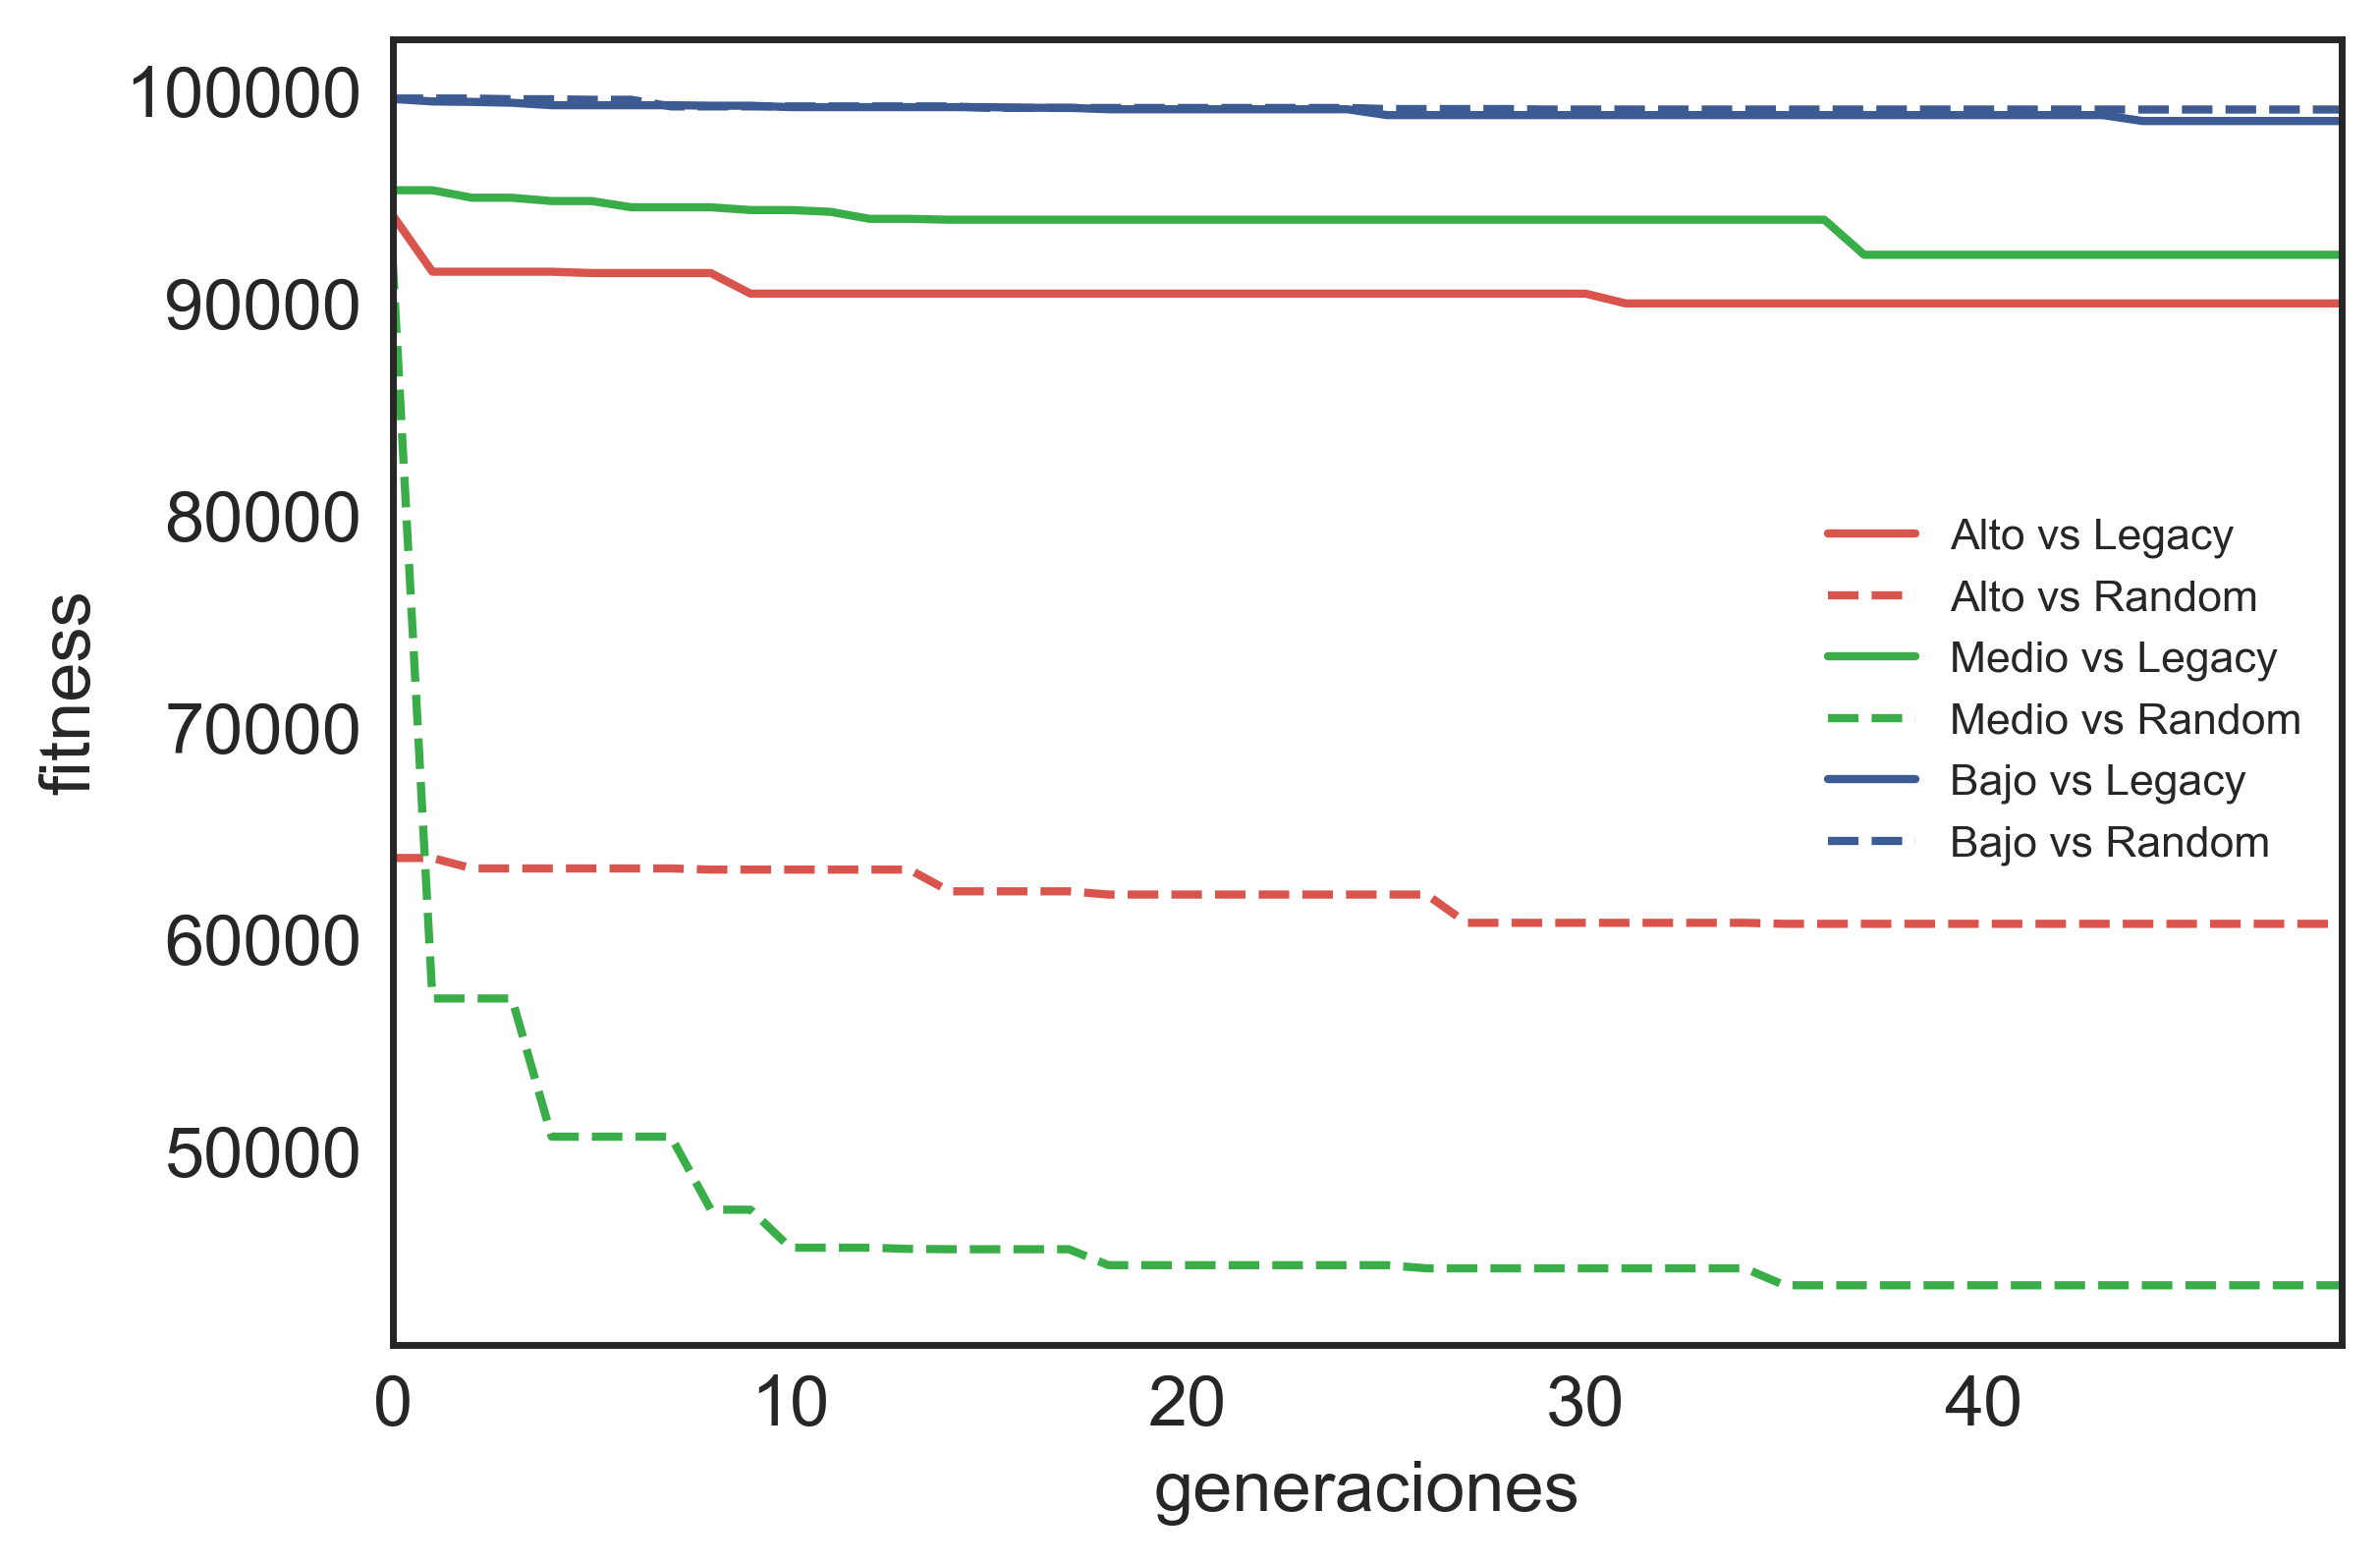
\includegraphics[width=0.8\textwidth]{grafica/all_fitnesses}
\label{graph:all_fitness}
\caption{\textit{Fitness} con un solo objetivo.}
\end{figure}

Segundo, tal como se aprecia se en la Figura~\ref{graph:all_fitness}, los bots consiguen mejores resultados en evoluciones con pocas generaciones, 50 en el caso de la gráfica, cuanto mayor es la abstracción de la gramática aplicada. No obstante, los bots generados usando la gramática de medio nivel consiguen superar a los de alto nivel con muchas generaciones (por ejemplo 100), al tener mayor potencial, como se explica más adelante en la Tabla~\ref{table:single_obj}.
 
Tercero, tal como se aprecia en la Tabla~\ref{table:single_obj}, los bots generados usando tanto la gramática de medio nivel como la de alto nivel superan los controladores de Pac-Man base así como otros bots generados por gramáticas evolutivas, como por ejemplo el generado por la universidad UCD de Dublín. Esto ocurre tanto enfrentándose al controlador \textit{Random Ghosts} como al de \textit{Legacy Ghosts}.
 
Uno de los factores que nos permiten obtener mejores resultados que el bot \cite{galvan2010evolving} de UCD Dublin (especialmente interesante al estar también basado en gramáticas evolutivas) consiste en que su bot emplea funciones demasiado específicas, las cuales acaban limitando el comportamiento del bot, siendo una de ellas por ejemplo esperar a que los fantasmas se acerquen siempre que se encuentre al lado de una \textit{power pill}. 
Otro de los factores es el uso de numerosos parámetros para evaluar sus funciones condicionales. Por ejemplo, su bot utiliza una ventana alrededor de Pac-Man, dentro de la cual evalúa condiciones como encontrar fantasmas dentro de esta. Para emplear dicha ventana, emplea dos parámetros ancho y alto. Por otro lado, nuestras funciones condicionales obtienen directamente la distancia de la ruta a determinados elementos, pudiendo operar esta distancia con distintos operadores numéricos sobre valores también numericos.
\begin{sidewaystable}[]
\centering
\label{table:single_obj}
\begin{tabular}{|l|c|r|r|r|r|r|r|r|r|r|}
\hline
\multicolumn{1}{|c|}{\multirow{2}{*}{\textbf{Pac-Man}}} & \multirow{2}{*}{\textbf{Ghosts}} & \multicolumn{3}{c|}{\textbf{score}} & \multicolumn{3}{c|}{\textbf{level}} & \multicolumn{3}{c|}{\textbf{time (game ticks)}} \\ \cline{3-11} 
\multicolumn{1}{|c|}{} &  & \multicolumn{1}{c|}{\textbf{max}} & \multicolumn{1}{c|}{\textbf{avg}} & \multicolumn{1}{c|}{\textbf{std}} & \multicolumn{1}{c|}{\textbf{max}} & \multicolumn{1}{c|}{\textbf{avg}} & \multicolumn{1}{c|}{\textbf{std}} & \multicolumn{1}{c|}{\textbf{max}} & \multicolumn{1}{c|}{\textbf{avg}} & \multicolumn{1}{c|}{\textbf{std}} \\ \hline
Random &  \multirow{5}{*}{Random} & 1380 & 501 & 213 & 1 & 0.036 & 0.186 & 5635 & 1943 & 887.5 \\ \cline{1-1} \cline{3-11} 
NearestPill &  & 18910 & 4471 & 2654 & 5 & 1 & 0.9 & 7216 & 1795 & 1018 \\ \cline{1-1} \cline{3-11} 
UCD Dublin bot \cite{galvan2010evolving} &  & 11640 & 4288 & - & - & - & - & - & - & - \\ \cline{1-1} \cline{3-11} 
\textbf{Low-level} &  & \textbf{900} & \textbf{151} & \textbf{117} & \textbf{1} & \textbf{0.071} & \textbf{0.257} & \textbf{5094} & \textbf{2151} & \textbf{972.1} \\ \cline{1-1} \cline{3-11} 
\textbf{Medium-level} &  & \textbf{64600} & \textbf{48558} & \textbf{10780} & \textbf{18} & \textbf{15} & \textbf{3.4} & \textbf{24000} & \textbf{21579} & \textbf{4470} \\ \cline{1-1} \cline{3-11} 
\textbf{High-level} &  & \textbf{55480} & \textbf{32704} & \textbf{13237} & \textbf{18} & \textbf{10.4} & \textbf{4.3} & \textbf{24000} & \textbf{17457} & \textbf{6784} \\ \hline
Random & \multirow{5}{*}{Legacy} & 1840 & 197 & 107 & 0 & 0 & 0 & 877 & 465 & 61.3 \\ \cline{1-1} \cline{3-11} 
NearestPill &  & 7190 & 3531 & 638 & 1 & 0.4 & 0.5 & 1881 & 1152 & 143.7 \\ \cline{1-1} \cline{3-11} 
UCD Dublin bot \cite{galvan2010evolving} &  & 12350 & 3945 & - & - & - & - & - & - & - \\ \cline{1-1} \cline{3-11} 
\textbf{Low-level} &  & \textbf{120} & \textbf{120} & \textbf{0} & \textbf{0} & \textbf{0} & \textbf{0} & \textbf{600} & \textbf{425} & \textbf{34.5} \\ \cline{1-1} \cline{3-11} 
\textbf{Medium-level} &  & \textbf{15960} & \textbf{6358} & \textbf{2883} & \textbf{3} & \textbf{0.9} & \textbf{0.7} & \textbf{4973} & \textbf{1916} & \textbf{730} \\ \cline{1-1} \cline{3-11} 
\textbf{High-level} &  & \textbf{20040} & \textbf{5972} & \textbf{2832} & \textbf{4} & \textbf{1} & \textbf{0.6} & \textbf{8364} & \textbf{2026} & \textbf{1020} \\ \hline
\end{tabular}
\caption{Pac-Man vs Ghost controllers' comparison.}
\end{sidewaystable}

Por último, si bien el empleo de la optimización multiobjetivo supone una mejora significativa en ejecuciones del algoritmo evolutivo relativamente cortas (al evitar estancamiento en los numerosos mínimos locales), no produce una diferencia suficientemente significativa en los bots generados mediante ejecuciones suficientemente largas. Esto es apreciable en la Tabla~\ref{table:multi-objective} (donde las sigles MO se refieren a los bots que emplean la Optimización Multiobjetivo), y sucede así en el caso concreto de Ms. Pac-Man vs Ghost debido a la relación directa entre los distintos fitness que hemos perseguido en multiobjetivo (fantasmas comidos, niveles completados y puntos alcanzados sin el multiplicador de puntos al comer fantasmas) con la puntuación (fitness perseguido previo a la optimización multiobjetivo), siendo esta una composición de los fitness anteriores.

\begin{sidewaystable}[]
\centering
\label{table:multi-objective}
\begin{tabular}{|l|c|r|r|r|r|r|r|r|r|r|}
\hline
\multicolumn{1}{|c|}{\multirow{2}{*}{\textbf{Pac-Man}}} & \multirow{2}{*}{\textbf{Ghosts}} & \multicolumn{3}{c|}{\textbf{score}} & \multicolumn{3}{c|}{\textbf{level}} & \multicolumn{3}{c|}{\textbf{time (game ticks)}} \\ \cline{3-11} 
\multicolumn{1}{|c|}{} &  & \multicolumn{1}{c|}{\textbf{max}} & \multicolumn{1}{c|}{\textbf{avg}} & \multicolumn{1}{c|}{\textbf{std}} & \multicolumn{1}{c|}{\textbf{max}} & \multicolumn{1}{c|}{\textbf{avg}} & \multicolumn{1}{c|}{\textbf{std}} & \multicolumn{1}{c|}{\textbf{max}} & \multicolumn{1}{c|}{\textbf{avg}} & \multicolumn{1}{c|}{\textbf{std}} \\ \hline
Medium-level \ref{table:single_obj} & \multirow{4}{*}{Random} & {64600} & {48558} & {10780} & {18} & {15} & {3.4} & {24000} & {21579} & {4470} \\ \cline{1-1} \cline{3-11} 
\textbf{Medium-level (MO)} &  & \textbf{62050} & \textbf{46922} & \textbf{1243} & \textbf{18} & \textbf{15} & \textbf{4} & \textbf{24000} & \textbf{20868} & \textbf{5094.5} \\ \cline{1-1} \cline{3-11} 
{High-level \ref{table:single_obj}} &  & {55480} & {32704} & {13237} & {18} & {10.4} & {4.3} & {24000} & {17457} & {6784} \\ \cline{1-1} \cline{3-11} 
\textbf{High-level (MO)} &  & \textbf{57370} & \textbf{32441} & \textbf{12712} & \textbf{17} & \textbf{10} & \textbf{4.1} & \textbf{24000} & \textbf{17536} & \textbf{6604.7} \\ \hline
{Medium-level \ref{table:single_obj}} & \multirow{4}{*}{Legacy} & {15960} & {6358} & {2883} & {3} & {0.9} & {0.7} & {4973} & {1916} & {730} \\ \cline{1-1} \cline{3-11} 
\textbf{Medium-level (MO)} &  & \textbf{18020} & \textbf{6229} & \textbf{2832} & \textbf{3} & \textbf{0.9} & \textbf{0.7} & \textbf{5041} & \textbf{1905} & \textbf{725} \\ \cline{1-1} \cline{3-11} 
{High-level \ref{table:single_obj}} &  & {20040} & {5972} & {2832} & {4} & {1} & {0.6} & {8364} & {2026} & {1020} \\ \cline{1-1} \cline{3-11} 
\textbf{High-level (MO)} &  & \textbf{20040} & \textbf{5972} & \textbf{2832} & \textbf{4} & \textbf{1} & \textbf{0.6} & \textbf{8364} & \textbf{2026} & \textbf{1020} \\ \hline
\end{tabular}
\caption{Pac-Man vs Ghost controllers' comparison including Multi-Objective.}
\end{sidewaystable}

\section{Difusión} \label{cap:paper}
Considerando el impacto que puede tener el proyecto que hemos realizado, hemos decidido publicarlo \cite{thesisGit} como código abierto y bajo licencia GPL \cite{licenseThesisGit} en la plataforma GitHub. Esto lo hicimos con la esperanza de poder ser de ayuda a cualquier proyecto relacionado con el campo de la evolución gramatical o la inteligencia artificial aplicada a videojuegos.

Finalmente, una vez habíamos obtenido y analizado los resultados del proyecto, decidimos llevarlo un paso mas allá y publicar un artículo científico sobre él. Este, titulado ``A Pac-Man bot based on Grammatical evolution'', se centra en la implementación final (arboles de decisión) y el uso de gramáticas de medio y alto nivel, mencionando brevemente la mejora de optimización multiobjetivo. En estos momentos el artículo ha sido enviado al CoSECiVi 2017 (Congreso de la Sociedad Española para las Ciencias del Videojuego) y se encuentra pendiente de revisión por pares.

\section{Trabajo futuro}
Aunque estamos satisfechos con el alcance de nuestro trabajo y sus resultados, nos habría gustado experimentar y comprobar otras técnicas no incluidas por falta de tiempo. Son las que se describen a continuación.

\subsection{Árboles de comportamiento}
Una de las posibles técnicas a aplicar son los árboles de comportamiento (\textit{Behaviour trees}). 
El uso de árboles de comportamiento habría supuesto incluir en nuestras gramáticas bucles en los formatos típicos (\texttt{while, for, do-while}, ...). Esto supone que para encontrar un terminal que devuelva un movimiento en nuestro árbol de decisión, ya no se parte siempre desde la raíz, sino que puede tener que continuarse en un punto definido por las solicitudes de movimiento previas.

Esta técnica en principio posibilita, o facilita la producción de estrategias más específicas, que requieran continuidad. Sin árboles de comportamiento también pueden conseguirse, pero el conjunto de condiciones a evaluar para llegar a dichas estrategias y soportar varias a la vez puede hacerse enorme, y llegar a dichas soluciones en un espacio de búsqueda tan grande/complejo es extremadamente poco factible en términos de potencia computacional.

\subsection{NEAT}
Otra técnica prometedora sería la aplicación de redes neuronales debido a su amplio espectro y gran capacidad de generalización.

Como \textit{input}s tendríamos las mismas funciones de las que hacen uso las gramáticas para conocer el estado del juego y como \textit{output} nos daría un movimiento que ejecutaría Pac-Man.

El problema radicaría en la arquitectura de la red, por lo que para dar con la óptima y siguiendo con el espíritu evolucionista, usaríamos el algoritmo NEAT \cite{stanley2002evolving} (\textit{NeuroEvolution of Augmenting Topologies}). Este algoritmo se vale de técnicas de Programación Evolutiva para evolucionar y proteger las topologías de las redes neuronales que genera hasta que están lo suficientemente entrenadas para resolver con éxito un problema concreto. La ventaja adicional es que se podría integrar dentro del framework JECO con mínimo esfuerzo, más allá de la implementación del mismo.